% Created by tikzDevice version 0.12.3.1 on 2021-06-15 13:45:43
% !TEX encoding = UTF-8 Unicode
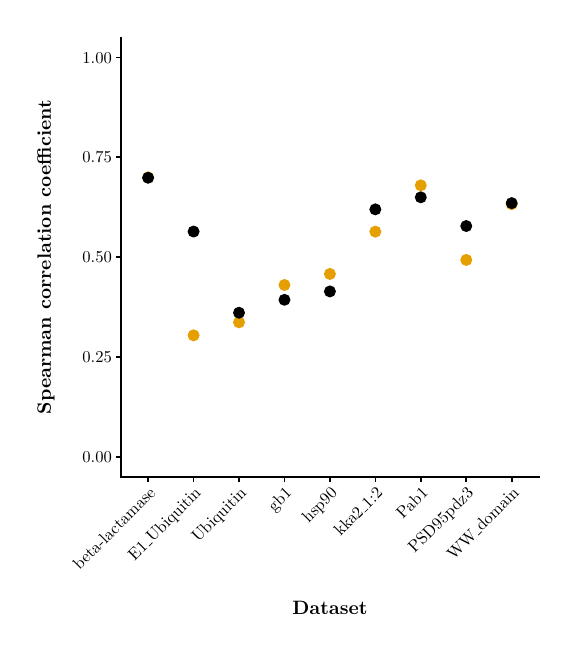
\begin{tikzpicture}[x=1pt,y=1pt]
\definecolor{fillColor}{RGB}{255,255,255}
\path[use as bounding box,fill=fillColor,fill opacity=0.00] (0,0) rectangle (188.25,216.81);
\begin{scope}
\path[clip] ( 33.67, 54.47) rectangle (184.75,213.31);
\definecolor{drawColor}{RGB}{230,159,0}
\definecolor{fillColor}{RGB}{230,159,0}

\path[draw=drawColor,line width= 0.4pt,line join=round,line cap=round,fill=fillColor] (125.63,143.10) circle (  1.96);
\definecolor{drawColor}{RGB}{0,0,0}
\definecolor{fillColor}{RGB}{0,0,0}

\path[draw=drawColor,line width= 0.4pt,line join=round,line cap=round,fill=fillColor] (125.63,151.16) circle (  1.96);
\definecolor{drawColor}{RGB}{230,159,0}
\definecolor{fillColor}{RGB}{230,159,0}

\path[draw=drawColor,line width= 0.4pt,line join=round,line cap=round,fill=fillColor] (109.21,127.82) circle (  1.96);
\definecolor{drawColor}{RGB}{0,0,0}
\definecolor{fillColor}{RGB}{0,0,0}

\path[draw=drawColor,line width= 0.4pt,line join=round,line cap=round,fill=fillColor] (109.21,121.50) circle (  1.96);
\definecolor{drawColor}{RGB}{230,159,0}
\definecolor{fillColor}{RGB}{230,159,0}

\path[draw=drawColor,line width= 0.4pt,line join=round,line cap=round,fill=fillColor] (142.05,159.84) circle (  1.96);
\definecolor{drawColor}{RGB}{0,0,0}
\definecolor{fillColor}{RGB}{0,0,0}

\path[draw=drawColor,line width= 0.4pt,line join=round,line cap=round,fill=fillColor] (142.05,155.51) circle (  1.96);
\definecolor{drawColor}{RGB}{230,159,0}
\definecolor{fillColor}{RGB}{230,159,0}

\path[draw=drawColor,line width= 0.4pt,line join=round,line cap=round,fill=fillColor] ( 92.79,123.83) circle (  1.96);
\definecolor{drawColor}{RGB}{0,0,0}
\definecolor{fillColor}{RGB}{0,0,0}

\path[draw=drawColor,line width= 0.4pt,line join=round,line cap=round,fill=fillColor] ( 92.79,118.47) circle (  1.96);
\definecolor{drawColor}{RGB}{230,159,0}
\definecolor{fillColor}{RGB}{230,159,0}

\path[draw=drawColor,line width= 0.4pt,line join=round,line cap=round,fill=fillColor] ( 76.37,110.34) circle (  1.96);

\path[draw=drawColor,line width= 0.4pt,line join=round,line cap=round,fill=fillColor] ( 59.95,105.63) circle (  1.96);
\definecolor{drawColor}{RGB}{0,0,0}
\definecolor{fillColor}{RGB}{0,0,0}

\path[draw=drawColor,line width= 0.4pt,line join=round,line cap=round,fill=fillColor] ( 76.37,113.80) circle (  1.96);

\path[draw=drawColor,line width= 0.4pt,line join=round,line cap=round,fill=fillColor] ( 59.95,143.14) circle (  1.96);
\definecolor{drawColor}{RGB}{230,159,0}
\definecolor{fillColor}{RGB}{230,159,0}

\path[draw=drawColor,line width= 0.4pt,line join=round,line cap=round,fill=fillColor] (158.48,132.88) circle (  1.96);
\definecolor{drawColor}{RGB}{0,0,0}
\definecolor{fillColor}{RGB}{0,0,0}

\path[draw=drawColor,line width= 0.4pt,line join=round,line cap=round,fill=fillColor] (158.48,145.13) circle (  1.96);
\definecolor{drawColor}{RGB}{230,159,0}
\definecolor{fillColor}{RGB}{230,159,0}

\path[draw=drawColor,line width= 0.4pt,line join=round,line cap=round,fill=fillColor] (174.90,153.04) circle (  1.96);
\definecolor{drawColor}{RGB}{0,0,0}
\definecolor{fillColor}{RGB}{0,0,0}

\path[draw=drawColor,line width= 0.4pt,line join=round,line cap=round,fill=fillColor] (174.90,153.41) circle (  1.96);
\definecolor{drawColor}{RGB}{230,159,0}
\definecolor{fillColor}{RGB}{230,159,0}

\path[draw=drawColor,line width= 0.4pt,line join=round,line cap=round,fill=fillColor] ( 43.52,162.71) circle (  1.96);
\definecolor{drawColor}{RGB}{0,0,0}
\definecolor{fillColor}{RGB}{0,0,0}

\path[draw=drawColor,line width= 0.4pt,line join=round,line cap=round,fill=fillColor] ( 43.52,162.57) circle (  1.96);
\end{scope}
\begin{scope}
\path[clip] (  0.00,  0.00) rectangle (188.25,216.81);
\definecolor{drawColor}{RGB}{0,0,0}

\path[draw=drawColor,line width= 0.6pt,line join=round,line cap=rect] ( 33.67, 54.47) --
	( 33.67,213.31);
\end{scope}
\begin{scope}
\path[clip] (  0.00,  0.00) rectangle (188.25,216.81);
\definecolor{drawColor}{RGB}{0,0,0}

\node[text=drawColor,anchor=base east,inner sep=0pt, outer sep=0pt, scale=  0.60] at ( 30.42, 59.62) {0.00};

\node[text=drawColor,anchor=base east,inner sep=0pt, outer sep=0pt, scale=  0.60] at ( 30.42, 95.72) {0.25};

\node[text=drawColor,anchor=base east,inner sep=0pt, outer sep=0pt, scale=  0.60] at ( 30.42,131.82) {0.50};

\node[text=drawColor,anchor=base east,inner sep=0pt, outer sep=0pt, scale=  0.60] at ( 30.42,167.92) {0.75};

\node[text=drawColor,anchor=base east,inner sep=0pt, outer sep=0pt, scale=  0.60] at ( 30.42,204.02) {1.00};
\end{scope}
\begin{scope}
\path[clip] (  0.00,  0.00) rectangle (188.25,216.81);
\definecolor{drawColor}{RGB}{0,0,0}

\path[draw=drawColor,line width= 0.6pt,line join=round] ( 31.92, 61.69) --
	( 33.67, 61.69);

\path[draw=drawColor,line width= 0.6pt,line join=round] ( 31.92, 97.79) --
	( 33.67, 97.79);

\path[draw=drawColor,line width= 0.6pt,line join=round] ( 31.92,133.89) --
	( 33.67,133.89);

\path[draw=drawColor,line width= 0.6pt,line join=round] ( 31.92,169.99) --
	( 33.67,169.99);

\path[draw=drawColor,line width= 0.6pt,line join=round] ( 31.92,206.09) --
	( 33.67,206.09);
\end{scope}
\begin{scope}
\path[clip] (  0.00,  0.00) rectangle (188.25,216.81);
\definecolor{drawColor}{RGB}{0,0,0}

\path[draw=drawColor,line width= 0.6pt,line join=round,line cap=rect] ( 33.67, 54.47) --
	(184.75, 54.47);
\end{scope}
\begin{scope}
\path[clip] (  0.00,  0.00) rectangle (188.25,216.81);
\definecolor{drawColor}{RGB}{0,0,0}

\path[draw=drawColor,line width= 0.6pt,line join=round] ( 43.52, 52.72) --
	( 43.52, 54.47);

\path[draw=drawColor,line width= 0.6pt,line join=round] ( 59.95, 52.72) --
	( 59.95, 54.47);

\path[draw=drawColor,line width= 0.6pt,line join=round] ( 76.37, 52.72) --
	( 76.37, 54.47);

\path[draw=drawColor,line width= 0.6pt,line join=round] ( 92.79, 52.72) --
	( 92.79, 54.47);

\path[draw=drawColor,line width= 0.6pt,line join=round] (109.21, 52.72) --
	(109.21, 54.47);

\path[draw=drawColor,line width= 0.6pt,line join=round] (125.63, 52.72) --
	(125.63, 54.47);

\path[draw=drawColor,line width= 0.6pt,line join=round] (142.05, 52.72) --
	(142.05, 54.47);

\path[draw=drawColor,line width= 0.6pt,line join=round] (158.48, 52.72) --
	(158.48, 54.47);

\path[draw=drawColor,line width= 0.6pt,line join=round] (174.90, 52.72) --
	(174.90, 54.47);
\end{scope}
\begin{scope}
\path[clip] (  0.00,  0.00) rectangle (188.25,216.81);
\definecolor{drawColor}{RGB}{0,0,0}

\node[text=drawColor,rotate= 45.00,anchor=base east,inner sep=0pt, outer sep=0pt, scale=  0.60] at ( 46.45, 48.30) {beta-lactamase};

\node[text=drawColor,rotate= 45.00,anchor=base east,inner sep=0pt, outer sep=0pt, scale=  0.60] at ( 62.87, 48.30) {E1\_Ubiquitin};

\node[text=drawColor,rotate= 45.00,anchor=base east,inner sep=0pt, outer sep=0pt, scale=  0.60] at ( 79.29, 48.30) {Ubiquitin};

\node[text=drawColor,rotate= 45.00,anchor=base east,inner sep=0pt, outer sep=0pt, scale=  0.60] at ( 95.71, 48.30) {gb1};

\node[text=drawColor,rotate= 45.00,anchor=base east,inner sep=0pt, outer sep=0pt, scale=  0.60] at (112.13, 48.30) {hsp90};

\node[text=drawColor,rotate= 45.00,anchor=base east,inner sep=0pt, outer sep=0pt, scale=  0.60] at (128.56, 48.30) {kka2\_1:2};

\node[text=drawColor,rotate= 45.00,anchor=base east,inner sep=0pt, outer sep=0pt, scale=  0.60] at (144.98, 48.30) {Pab1};

\node[text=drawColor,rotate= 45.00,anchor=base east,inner sep=0pt, outer sep=0pt, scale=  0.60] at (161.40, 48.30) {PSD95pdz3};

\node[text=drawColor,rotate= 45.00,anchor=base east,inner sep=0pt, outer sep=0pt, scale=  0.60] at (177.82, 48.30) {WW\_domain};
\end{scope}
\begin{scope}
\path[clip] (  0.00,  0.00) rectangle (188.25,216.81);
\definecolor{drawColor}{RGB}{0,0,0}

\node[text=drawColor,anchor=base,inner sep=0pt, outer sep=0pt, scale=  0.70] at (109.21,  4.86) {\bfseries Dataset};
\end{scope}
\begin{scope}
\path[clip] (  0.00,  0.00) rectangle (188.25,216.81);
\definecolor{drawColor}{RGB}{0,0,0}

\node[text=drawColor,rotate= 90.00,anchor=base,inner sep=0pt, outer sep=0pt, scale=  0.70] at (  8.39,133.89) {\bfseries Spearman correlation coefficient};
\end{scope}
\end{tikzpicture}%
